\chapter{Data analysis}\label{sec:data-ana}

Data is the essential part of a machine learning model.
Therefore, a wisely chosen dataset is needed.
The dataset used in this thesis is the Indoor Location \& Navigation from kaggle\cite{kaggle} which was part of a competition of Microsoft Research in 2021\cite{IndoorLocationNavigation}.
The data was recorded in shopping malls by a company called XYZ\(^{10}\) and was provided by Microsoft Research for this competition.
The goal for the competition was, given a site-path file, predict the floor and waypoint locations at a timestamp given in the submission files.


\section{Components of the dataset}\label{sec:data}
As noted in the kaggle notebook ``Indoor Navigation: Complete Data Understanding''\cite{IndoorNavigationUnderstanding} the data consists of 3 parts:
% 
\begin{itemize}
    \item a train folder with train path files, organized by site and floor
    \item a test folder with test path files, organized by site and floor but without waypoint data
    \item a metadata folder with floor metadata, organized by site and floor, which includes floor images, further information and a geojson map
\end{itemize}

For this thesis, the submission files as well as the test folder will not be used, because our goal is another type of prediction.
In the following, the train folder will be analyzed.
In general every file was hashed, so that no specific information about the site is visible.
The train folder consists of 204 subfolders, which represent each site where the data was recorded.
In each site folder are a minimum of one and a maximum twelve subfolders, which represent the floors of the site, the median is 5 floors.
Overall there are 26,925 files each representing a movement on a specific floor and site.
Per floor, there are between one and 284 files with a median of 14 files.
These files contain the information about the movement of a person on this specific site and floor.
With this amount of data, it could be possible to train a machine learning model.


\section{File structure}\label{sec:file-structure}
Each file contains the following information:
% do not use this, it's ugly
% \begin{figure}[h]
% 	\centering
%   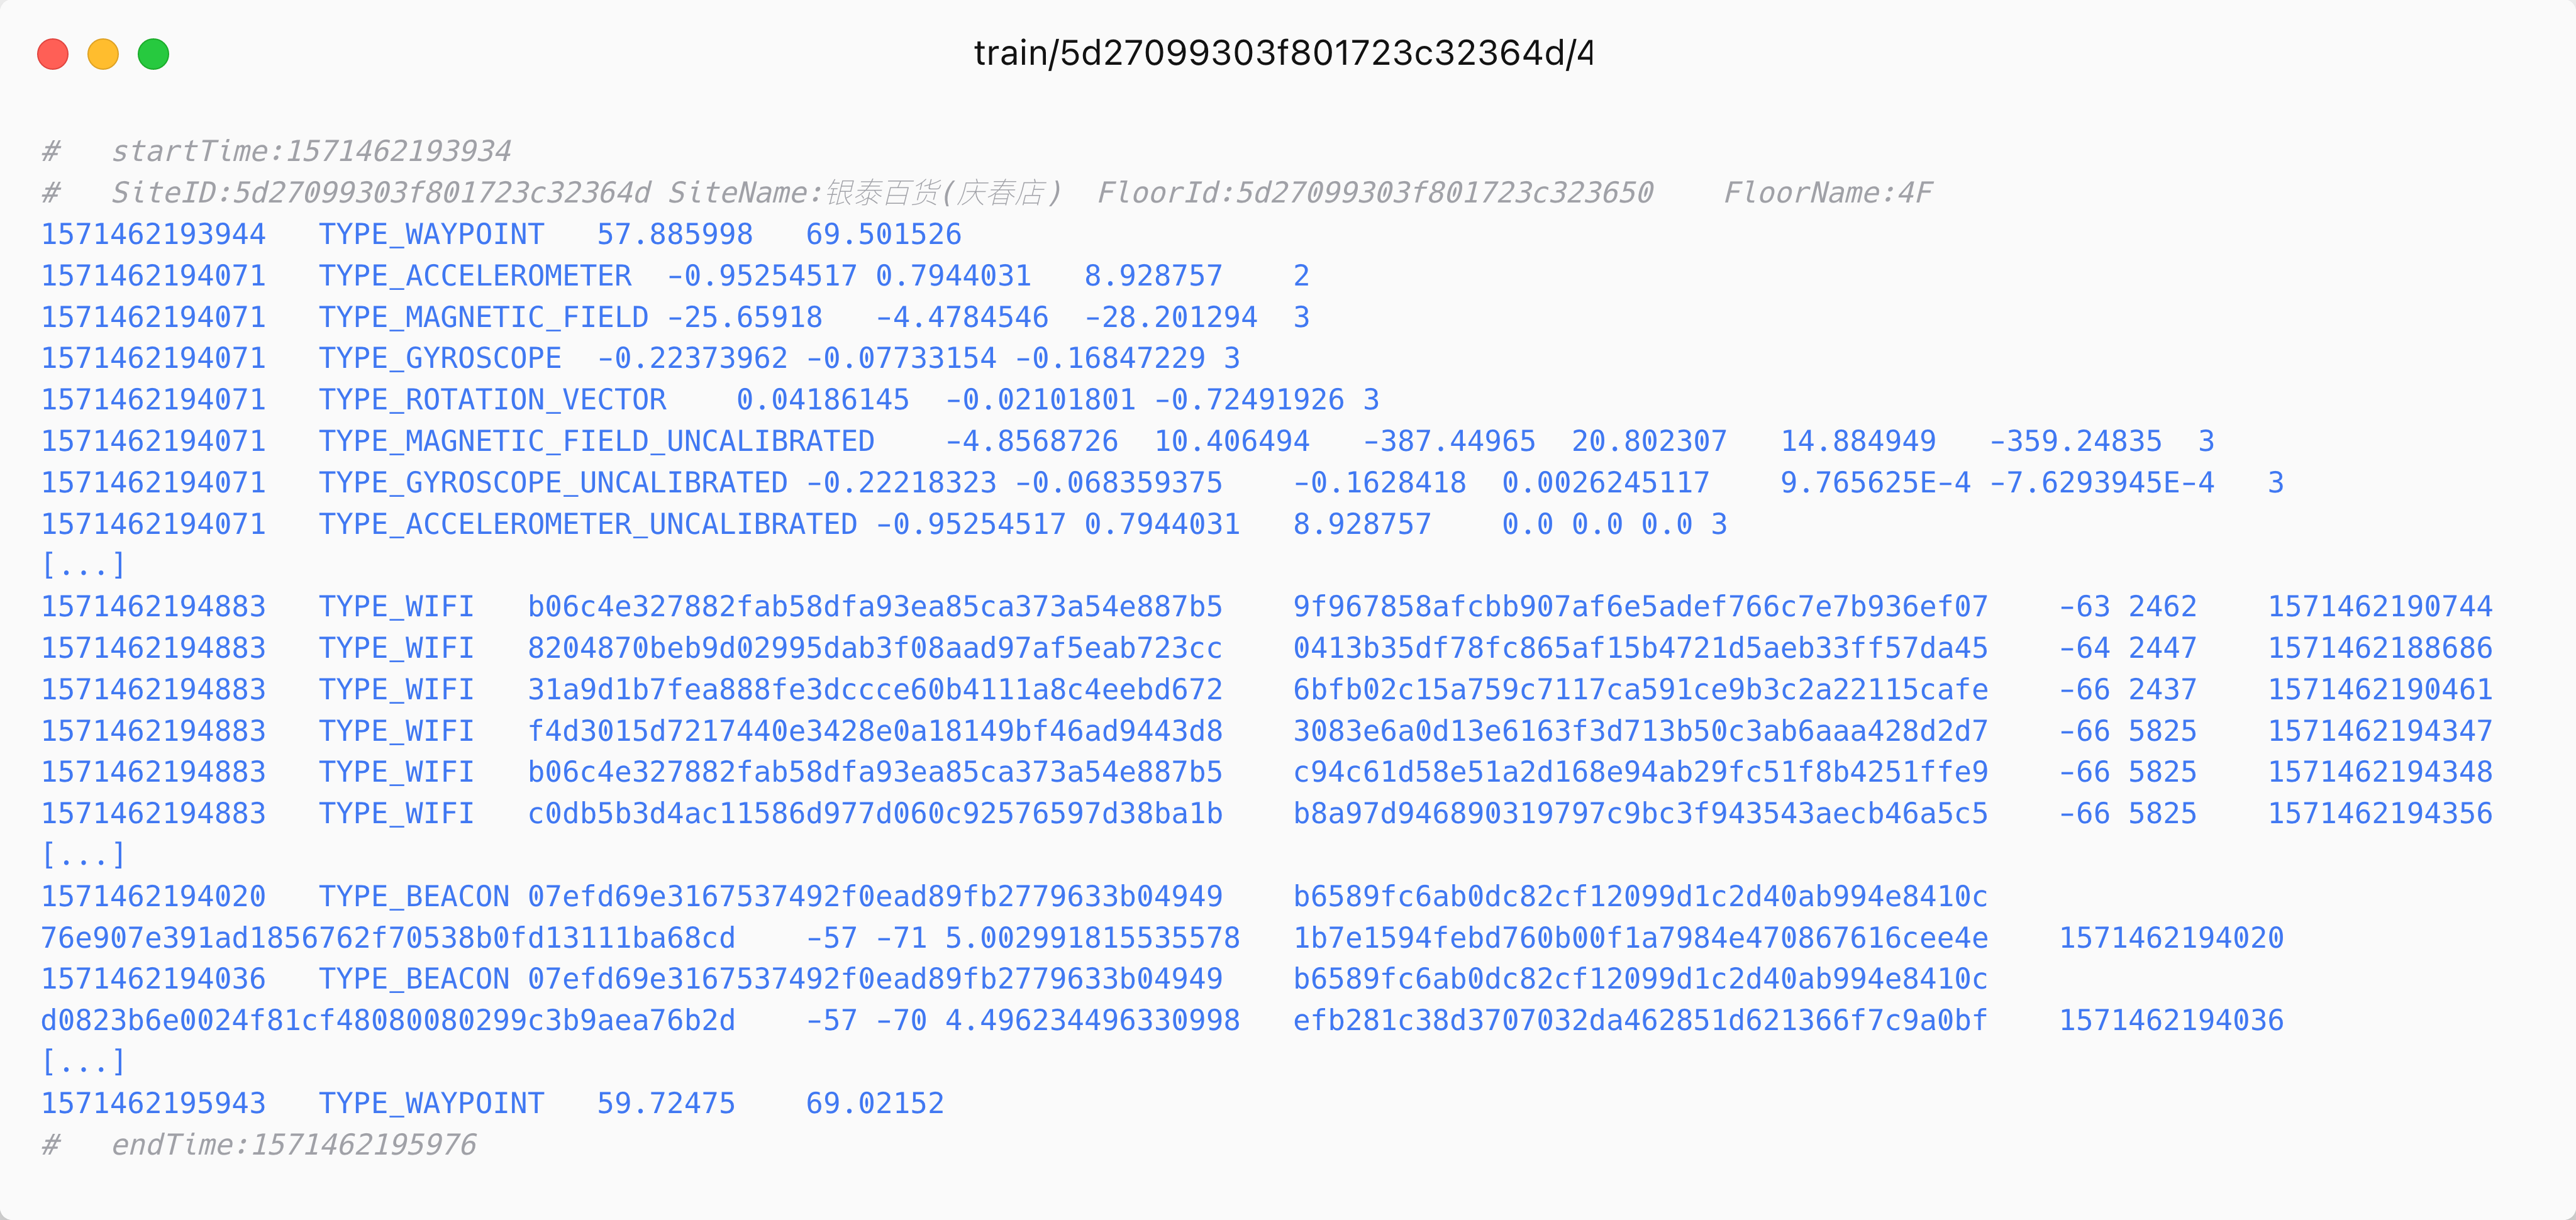
\includegraphics[angle=270,scale=0.15]{file-example.png}
% 	\caption{Each file includes X different }\label{fig:structure-data}
% \end{figure}



\lstset{
    basicstyle=\scriptsize\ttfamily,
    breaklines=true,
    escapeinside={(*@}{@*)},
}

\begin{lstlisting}
    \#	startTime:1571462193934
    \#	SiteID:5d27099303f801723c32364d	SiteName: (*@\begin{CJK*}{UTF8}{gbsn}银泰百货(庆春店)\end{CJK*}@*) FloorId:5d27099303f801723c323650	FloorName:4F
    1571462193944	TYPE_WAYPOINT	57.885998	69.501526
    1571462194071	TYPE_ACCELEROMETER	-0.95254517	0.7944031	8.928757	2
    1571462194071	TYPE_MAGNETIC_FIELD	-25.65918	-4.4784546	-28.201294	3
    1571462194071	TYPE_GYROSCOPE	-0.22373962	-0.07733154	-0.16847229	3
    1571462194071	TYPE_ROTATION_VECTOR	0.04186145	-0.02101801	-0.72491926	3
    1571462194071	TYPE_MAGNETIC_FIELD_UNCALIBRATED	-4.8568726	10.406494	-387.44965	20.802307	14.884949	-359.24835	3
    1571462194071	TYPE_GYROSCOPE_UNCALIBRATED	-0.22218323	-0.068359375	-0.1628418	0.0026245117	9.765625E-4	-7.6293945E-4	3
    1571462194071	TYPE_ACCELEROMETER_UNCALIBRATED	-0.95254517	0.7944031	8.928757	0.0	0.0	0.0	3
    ...
    1571462194883	TYPE_WIFI	b06c4e327882fab58dfa93ea85ca373a54e887b5	9f967858afcbb907af6e5adef766c7e7b936ef07	-63	2462	1571462190744
    1571462194883	TYPE_WIFI	8204870beb9d02995dab3f08aad97af5eab723cc	0413b35df78fc865af15b4721d5aeb33ff57da45	-64	2447	1571462188686
    ...
    1571462194020	TYPE_BEACON	07efd69e3167537492f0ead89fb2779633b04949	b6589fc6ab0dc82cf12099d1c2d40ab994e8410c	76e907e391ad1856762f70538b0fd13111ba68cd	-57	-71	5.002991815535578	1b7e1594febd760b00f1a7984e470867616cee4e	1571462194020
    ...
    \#	endTime:1571462195976
\end{lstlisting}





BSSIDs are hashed, so no original BSSIDs are visible

